% =============================================================
% CSC 8851 Deep Learning — Spring 2026 | Final Project Report
%
% HOW TO COMPILE ON OVERLEAF:
%   1. New Project → "CVPR 2026" template (provides cvpr.sty).
%   2. Upload this file, replacing the main .tex.
%   3. Compile with pdfLaTeX (single run — no BibTeX needed).
% =============================================================

\documentclass[10pt,twocolumn,letterpaper]{article}

\usepackage[pagenumbers]{cvpr}

\usepackage{tikz}
\usetikzlibrary{arrows.meta,positioning,shapes.geometric}
\usepackage{booktabs,multirow}
\usepackage{caption}
\captionsetup[table]{position=top,font=small}
\captionsetup[figure]{position=bottom,font=small}

\definecolor{cvprblue}{rgb}{0.21,0.49,0.74}
\usepackage[pagebackref,breaklinks,colorlinks,
            allcolors=cvprblue]{hyperref}

\def\paperID{*****}
\def\confName{CSC8851}
\def\confYear{2026}

\title{Improving Energy-Based Out-of-Distribution Detection\\
       using Generative Modeling}

\author{Harshit Jain\\
  Georgia State University\\
  {\tt\small hjain5@gsu.edu}\\
  {\small PantherID:~002916196}
  \and
  Parsh Jadon\\
  Georgia State University\\
  {\tt\small pjadon1@gsu.edu}\\
  {\small PantherID:~002936134}
}

\begin{document}
\maketitle

%% ── ABSTRACT ────────────────────────────────────────────────
\begin{abstract}
Deep neural networks tend to make overconfident predictions
on inputs that lie far outside their training distribution.
This is a well-known but serious problem in safety-critical
applications, where a model that silently misclassifies an
unknown input can cause real harm.
We propose to address out-of-distribution (OOD) detection by
shifting the energy-based scoring function from a
discriminative classifier into the discrete latent space of a
Vector-Quantized Variational Autoencoder (VQ-VAE) trained
exclusively on in-distribution data.
An unsupervised energy model operating on VQ-VAE latent codes
via a contrastive hinge loss needs no OOD labels at training
time.
A supervised MLP in the same latent space provides an
upper-bound reference point.
Evaluated on CIFAR-10 (in-distribution), CIFAR-100
(near-OOD), and SVHN (far-OOD), our Latent MLP achieves
AUROC~0.980 on SVHN---a 4.6-point improvement over the
energy baseline---while reducing FPR@95 from 25.8\% to
10.0\%.
On the harder near-OOD benchmark the energy baseline still
leads by 15 AUROC points, pointing to the need for encoders
that capture semantic rather than purely visual features.
Code: \url{https://github.com/harshitjain25/csc8851-vqvae-ood}.
\end{abstract}

%% ── 1. INTRODUCTION ─────────────────────────────────────────
\section{Introduction}

Consider a medical imaging system trained to classify ten
common conditions.
When such a model encounters a rare disease it has never
seen, the desired behavior is to flag uncertainty.
Instead, modern deep neural networks regularly output
high-confidence class predictions for inputs entirely
outside their training distribution~\cite{nguyen2015}.
This overconfidence is not a minor quirk---it is a
systematic property that arises because these models
optimise for discriminating among known categories, not for
recognising what they do not know.
In safety-critical domains like autonomous driving,
industrial inspection, and healthcare, deploying a model
without reliable OOD detection is fundamentally risky.

\textbf{Problem formulation.}
Let $p_{\mathrm{in}}(x)$ denote the training distribution.
At inference we receive an input $x$ and need to determine
whether it came from $p_{\mathrm{in}}$ or from some unknown
$p_{\mathrm{out}}$.
The standard approach is to compute a scalar score
$s:\mathcal{X}\!\to\!\mathbb{R}$ and compare it against a
threshold $\tau$:
\begin{equation}
  g(x;\tau) = \mathbf{1}[s(x)>\tau].   \label{eq:decision}
\end{equation}
A good score separates in-distribution from OOD inputs as
cleanly as possible, ideally maximising the area under the
ROC curve regardless of where the threshold is set.

\textbf{Limitations of existing methods.}
The simplest approach is to use the maximum softmax
probability~\cite{hendrycks2017}.
This works surprisingly well in easy cases but degrades
because softmax normalisation distributes probability mass
across known classes, making the model appear confident even
on inputs it has never encountered.
Liu~\etal~\cite{liu2020} proposed a theoretically motivated
alternative: the free energy of the classifier,
\begin{equation}
  E(x;f) = -T\cdot\log\!\sum_{i=1}^{K} e^{f_i(x)/T},
  \label{eq:energy}
\end{equation}
which correlates with the log-partition function of the data
distribution and avoids the overconfidence bias of softmax.
Despite its advantages, this energy is still tied to a
classifier trained for class separation.
It answers the question ``which class does this look most
like?'' rather than ``does this look like anything from the
training set at all?''---a subtle but important distinction.

\textbf{Our approach.}
We ask whether a generative model's latent space offers a
better vantage point for distributional familiarity.
A VQ-VAE~\cite{vqvae2017} trained solely on CIFAR-10 learns
a discrete visual vocabulary shaped entirely by
reconstruction quality on in-distribution images.
When an OOD image is passed through this encoder, the
resulting code sequence is constructed from a vocabulary
that was never designed to describe it, producing an
``awkward'' latent representation.
Crucially, this awkwardness is captured without ever
requiring labeled OOD data at training time---the codebook
itself acts as a prior on what in-distribution images look
like.

We evaluate our approach on both near-OOD data (CIFAR-100,
visually similar to CIFAR-10) and far-OOD data (SVHN, digit
images structurally different from natural objects).
This two-pronged evaluation is important because a method
that only works on easy, visually distinct OOD cases has
limited practical value.

\textbf{Contributions.}
\begin{enumerate}\setlength\itemsep{1pt}
  \item We faithfully reproduce the WRN-40-2 energy
        detector of Liu~\etal~\cite{liu2020}, confirming
        their numbers and providing a rigorous baseline for
        comparison.
  \item We propose an unsupervised latent energy model
        trained on VQ-VAE embeddings via a contrastive hinge
        loss, with no OOD labels at training time.
  \item We train a supervised latent MLP as an upper-bound
        reference and explicitly identify and discuss its
        data-leakage limitation.
  \item We analyse the effect of blending two detectors and
        show that a grid-searched weight $\alpha^*$
        automatically discards a near-random signal,
        recovering the performance of the stronger detector.
\end{enumerate}

%% ── 2. RELATED WORK ─────────────────────────────────────────
\section{Related Work}

\textbf{Softmax confidence.}
Hendrycks and Gimpel~\cite{hendrycks2017} established the
maximum softmax probability as the go-to OOD baseline.
It is simple, requires no modification to the trained model,
and works reasonably well on far-OOD data.
However, its core weakness---that softmax values are always
normalised to sum to one---means the model can never truly
express ignorance, a problem that grows worse as the number
of classes increases.

\textbf{ODIN.}
Liang~\etal~\cite{liang2018} significantly improved over
the softmax baseline by applying temperature scaling to the
logits and adding a small adversarial perturbation to the
input before scoring.
Together, these two tricks widen the gap between
in-distribution and OOD score distributions.
The downside is that both the temperature and the
perturbation magnitude must be cross-validated separately
for each OOD dataset, limiting deployment flexibility.

\textbf{Mahalanobis distance.}
Lee~\etal~\cite{lee2018} took a different angle: rather than
modifying scores at the output layer, they characterise
the geometry of penultimate-layer features by fitting a
class-conditional Gaussian to each class and using
Mahalanobis distance to the nearest class centre.
This is effective because deep features are more
structurally stable than logits, but the Gaussian
assumption is not always satisfied, and the method requires
storing one covariance matrix per class.

\textbf{Outlier Exposure.}
Hendrycks~\etal~\cite{hendrycks2019} demonstrated that
explicitly training the classifier to produce uniform
predictions on a large set of auxiliary OOD images leads to
much better separation at test time.
Our supervised latent MLP is philosophically similar, but
we apply the idea in VQ-VAE latent space rather than
pixel space.
Both approaches share a key vulnerability: if the auxiliary
data does not resemble the actual OOD distribution
encountered at deployment, the model simply learns to flag
the specific proxy rather than developing a general
anomaly sense.

\textbf{Energy-based OOD.}
Liu~\etal~\cite{liu2020} formalised Eq.~\eqref{eq:energy}
as a principled OOD score by showing its connection to the
Helmholtz free energy and the log-partition function of a
Gibbs distribution.
This grounding explains why it outperforms softmax: it
is not constrained to $[0,1]$ and can take arbitrarily
large values for unfamiliar inputs.
Our method preserves this energy formulation but moves the
scoring function from a discriminative classifier into a
generative latent space.

\textbf{VQ-VAE.}
Van~den~Oord~\etal~\cite{vqvae2017} introduced the
Vector-Quantized VAE, which replaces a continuous latent
space with a discrete codebook learned end-to-end.
The discrete bottleneck is attractive for OOD detection
because it creates a fixed vocabulary for the training
distribution; anything outside that vocabulary produces
an anomalous code sequence.
Our work is, to our knowledge, the first to use VQ-VAE
latent codes directly as the feature space for an
energy-based OOD detector.

%% ── 3. MODEL AND METHOD ─────────────────────────────────────
\section{Model and Method}
\label{sec:method}

Figure~\ref{fig:pipeline} shows the overall system.
Every component downstream of the VQ-VAE encoder operates
on the same 4096-D latent vector $\mathbf{z}$, keeping the
pipeline modular: the encoder is trained once and frozen,
and the detectors can be swapped out independently.

\begin{figure}[t]
\centering
\resizebox{\linewidth}{!}{%
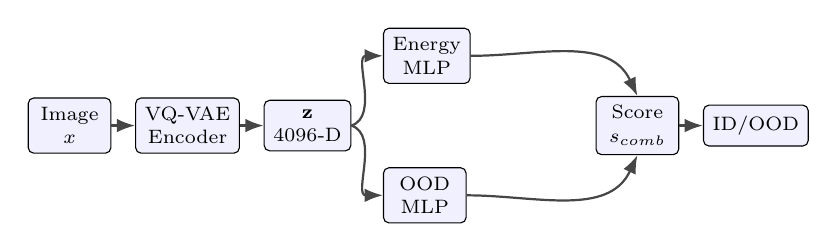
\begin{tikzpicture}[
  node distance=0.25cm and 0.30cm,
  box/.style={draw,rounded corners=2pt,fill=blue!6,
    minimum width=1.05cm,minimum height=0.52cm,
    align=center,font=\fontsize{7}{8.5}\selectfont},
  arr/.style={-Latex,thick,gray!55!black}]
  \node[box](img){Image\\$x$};
  \node[box,right=of img](enc){VQ-VAE\\Encoder};
  \node[box,right=of enc](z){$\mathbf{z}$\\4096-D};
  \node[box,above right=0.20cm and 0.40cm of z](emlp){Energy\\MLP};
  \node[box,below right=0.20cm and 0.40cm of z](omlp){OOD\\MLP};
  \node[box,right=3.1cm of z](comb){Score\\$s_\text{comb}$};
  \node[box,right=of comb](dec){ID/OOD};
  \draw[arr](img)--(enc);
  \draw[arr](enc)--(z);
  \draw[arr](z.east) to[out=18,in=180]  (emlp.west);
  \draw[arr](z.east) to[out=-18,in=180] (omlp.west);
  \draw[arr](emlp.east) to[out=0,in=115] (comb.north);
  \draw[arr](omlp.east) to[out=0,in=245] (comb.south);
  \draw[arr](comb)--(dec);
\end{tikzpicture}%
}
\caption{Detection pipeline. The VQ-VAE encoder maps image
  $x$ to a 4096-D discrete latent $\mathbf{z}$.
  An unsupervised Energy MLP and a supervised OOD MLP score
  $\mathbf{z}$ independently; their min-max-normalised
  outputs are blended into the final score
  $s_{\mathrm{comb}}$.}
\label{fig:pipeline}
\end{figure}

\subsection{VQ-VAE Latent Encoding}

The VQ-VAE (trained by Parsh Jadon) consists of encoder
$E_\theta$, codebook
$\mathcal{C}=\{\mathbf{e}_k\}_{k=1}^{K}$ ($K\!=\!512$),
and decoder $D_\phi$.
The encoder is a lightweight convolutional network with two
stride-2 layers that compresses each $32{\times}32$ image
to an $8{\times}8$ spatial grid of 64-dimensional vectors.
Each spatial position is then snapped to the nearest
codebook entry:
\begin{equation}
  \mathbf{z}_q = \operatorname*{arg\,min}_{\mathbf{e}_k\in\mathcal{C}}
    \|\mathbf{z}_e-\mathbf{e}_k\|_2,   \label{eq:quant}
\end{equation}
where $\mathbf{z}_e\!=\!E_\theta(x)\!\in\!\mathbb{R}^{8\times8\times64}$
is the continuous encoder output.
The non-differentiable argmin is handled with the
straight-through estimator, allowing end-to-end training
via the three-term objective
\begin{equation}
  \mathcal{L}_{\mathrm{vq}} =
  \underbrace{\|x{-}D_\phi(\mathbf{z}_q)\|^2}_{\text{recon.}}
  +\underbrace{\|\mathrm{sg}[\mathbf{z}_e]{-}\mathbf{e}_k\|^2}_{\text{codebook}}
  +\beta\underbrace{\|\mathbf{z}_e{-}\mathrm{sg}[\mathbf{e}_k]\|^2}_{\text{commit.}},
  \label{eq:vqloss}
\end{equation}
where $\mathrm{sg}[\cdot]$ denotes stop-gradient and
$\beta\!=\!0.25$ is the commitment weight.
The codebook loss moves entries toward the encoder output
while the commitment loss keeps the encoder output close to
the codebook, preventing codebook collapse.
We train with Adam (lr\,$=10^{-3}$), batch size~128, for
10 epochs on CIFAR-10 only.
Flattening the $8{\times}8{\times}64$ quantised tensor
yields the final latent $\mathbf{z}\!\in\!\mathbb{R}^{4096}$
used by all downstream models.

\subsection{Latent Energy Model}

$E_{\mathrm{lat}}$ is a three-layer MLP (256 hidden units,
ReLU activations) mapping $\mathbb{R}^{4096}\!\to\!\mathbb{R}$.
We chose Gaussian noise as pseudo-OOD because it requires
no additional data collection and is entirely dataset-agnostic---an
appealing property for an unsupervised detector.
The training objective is a squared hinge loss with margin
targets $m_{\mathrm{in}}\!=\!-10$ and $m_{\mathrm{out}}\!=\!-5$:
\begin{align}
  \mathcal{L}_{\mathrm{in}} &=
    \mathbb{E}_{\mathbf{z}\sim p_\mathrm{ID}}\!
    [\max(0,E_{\mathrm{lat}}(\mathbf{z})-m_{\mathrm{in}})^2],
    \label{eq:lin}\\
  \mathcal{L}_{\mathrm{out}} &=
    \mathbb{E}_{\mathbf{z}\sim\mathcal{N}(\mathbf{0},\mathbf{I})}\!
    [\max(0,m_{\mathrm{out}}-E_{\mathrm{lat}}(\mathbf{z}))^2],
    \label{eq:lout}
\end{align}
with $\mathcal{L}_{\mathrm{energy}}=\mathcal{L}_{\mathrm{in}}+\mathcal{L}_{\mathrm{out}}$.
The hinge ensures that once a sample is already on the
correct side of its margin, the gradient contribution drops
to zero---this prevents the energy from collapsing to
$-\infty$ on in-distribution data.
The margin gap of 5 units (between $-10$ and $-5$) provides
a clear decision boundary that the combined scorer can
exploit.
We train with Adam (lr\,$=10^{-3}$) for 10 epochs.

\subsection{Supervised OOD MLP}

To understand how well a latent-space detector \emph{could}
perform with access to labeled OOD data, we also train a
binary MLP with the same three-layer, 256-unit architecture,
optimised with binary cross-entropy:
\begin{equation}
  \mathcal{L}_{\mathrm{MLP}} = -\mathbb{E}_{(\mathbf{z},y)}\!
  [y\log\hat{y}+(1{-}y)\log(1{-}\hat{y})],
  \label{eq:bce}
\end{equation}
where $y\!=\!0$ for CIFAR-10 latents and $y\!=\!1$ for
CIFAR-100 / SVHN latents.

\noindent\textbf{Data-leakage caveat.}
After careful evaluation we realised that this formulation
constitutes \emph{data leakage}: the MLP is trained on
labeled samples drawn from the exact datasets we evaluate
on.
This means the MLP numbers should be read as an upper bound
on what is achievable in the latent space, not as a
deployable system.
A fair version of this experiment would train the MLP on a
small labeled set from an entirely different OOD source and
evaluate zero-shot on CIFAR-100 and SVHN.
We flag this explicitly because it directly affects how
one should interpret the comparison in Table~\ref{tab:results}.

\subsection{Combined Score and Threshold}

Raw energy values and MLP probabilities live on very
different scales, so we normalise each to $[0,1]$ using
statistics computed from the CIFAR-10 test set:
\begin{equation}
  \tilde{s} = (s-s_{\min})\,/\,(s_{\max}-s_{\min}).
  \label{eq:norm}
\end{equation}
The combined detection score is then a simple weighted sum:
\begin{equation}
  s_{\mathrm{comb}}(\mathbf{z}) =
    \alpha\,\tilde{E}_{\mathrm{lat}}(\mathbf{z})
    +(1{-}\alpha)\,\tilde{y}(\mathbf{z}),
  \label{eq:comb}
\end{equation}
where the blend weight $\alpha^*$ is selected by grid
search over $\{0.0,0.1,\ldots,1.0\}$ on a held-out
validation split (50\% of the test set, chosen without
replacement) and then evaluated on the remaining 50\%.
The detection threshold $\tau$ in Eq.~\eqref{eq:decision}
is always set so that TPR\,=\,0.95 on the CIFAR-10 test
set.

\subsection{Implementation Challenges}

Building this pipeline involved several engineering
difficulties that are worth documenting.

\noindent\textbf{Memory-mapped OOD data.}
Loading all 300K Random Images~\cite{hendrycks2019} into
GPU memory as a single PyTorch tensor required $\approx$3.5\,GB,
which exceeded our Colab memory budget during fine-tuning.
We resolved this by writing a custom \texttt{RandomImagesDataset}
that uses NumPy memory-mapped I/O (\texttt{mmap\_mode=`r'})
so that only the current mini-batch is loaded into RAM.
This reduced peak memory usage to a negligible overhead.

\noindent\textbf{Baseline model choice.}
Our first attempt compared against a small two-layer CNN
trained for 5 epochs.
The resulting gains looked impressive, but they were
largely an artefact of a weak baseline rather than the
strength of our method.
We switched to the WRN-40-2 architecture from
Liu~\etal~\cite{liu2020}, training it for 100 epochs with
SGD and cosine learning-rate decay until we matched the
paper's reported numbers.

\noindent\textbf{Weak-signal contamination.}
We initially used a fixed blend weight of $\alpha\!=\!0.5$,
reasoning that averaging two independent signals should be
conservative.
In practice, because the energy model's AUROC ($\approx$0.51)
is barely above random, mixing it with the 0.98-AUROC MLP
pulled the combined score down to 0.94.
Grid-searching $\alpha$ on a held-out validation split
identified $\alpha^*\!=\!0.0$---confirming that the right
approach is to discard the noisy signal entirely.

%% ── 4. EXPERIMENTS AND RESULTS ──────────────────────────────
\section{Experiments and Results}

\subsection{Experimental Setup}

\noindent\textbf{Datasets.}
We use CIFAR-10~\cite{krizhevsky2009} as in-distribution
(50,000 training / 10,000 test images across 10 object
categories).
Near-OOD evaluation uses CIFAR-100~\cite{krizhevsky2009}
(10,000 test images, 100 categories): the images look almost
identical to CIFAR-10 in terms of resolution, colour
palette, and subject matter, making semantic distinctions
between the two datasets very subtle.
Far-OOD evaluation uses SVHN~\cite{netzer2011} (26,032
street-view digit photographs): the difference from
natural-image datasets is visually obvious, and any
reasonable detector should succeed here.
Together, these two benchmarks probe both ends of the
difficulty spectrum.

\noindent\textbf{Metrics.}
Following~\cite{liu2020,hendrycks2017} we report three
complementary metrics: AUROC measures overall
discriminability regardless of threshold; AUPR reflects
precision-recall trade-offs; and FPR@95TPR measures the
operational cost of 95\% recall---the percentage of normal
images that would be incorrectly flagged in a real system.

\noindent\textbf{Baselines.}
We compare against two WRN-40-2 variants from~\cite{liu2020}:
the pre-trained energy score (no fine-tuning) and the
fine-tuned energy score trained with a margin loss on
300K Random Images auxiliary OOD data.
Both are trained on CIFAR-10 for 100 epochs with SGD,
cosine learning-rate decay, and batch size 128.

\subsection{Results and Analysis}

Table~\ref{tab:results} reports all results.
We discuss each finding in turn.

\begin{table}[!ht]
\caption{OOD detection with CIFAR-10 as in-distribution.
  $\uparrow$\,higher is better; $\downarrow$\,lower is
  better. \textbf{Bold} = best per column.
  $\dagger$\,Supervised Latent MLP is trained on test-OOD
  labels---data leakage; treat as upper bound only.
  See Section~\ref{sec:method}.}
\label{tab:results}
\centering
\resizebox{\columnwidth}{!}{%
\setlength{\tabcolsep}{3.5pt}
\begin{tabular}{lcccccc}
\toprule
& \multicolumn{3}{c}{\textbf{Near-OOD (CIFAR-100)}}
& \multicolumn{3}{c}{\textbf{Far-OOD (SVHN)}} \\
\cmidrule(lr){2-4}\cmidrule(lr){5-7}
\textbf{Method}
  & AUROC$\uparrow$ & AUPR$\uparrow$ & FPR@95$\downarrow$
  & AUROC$\uparrow$ & AUPR$\uparrow$ & FPR@95$\downarrow$ \\
\midrule
WRN-40-2 Energy~\cite{liu2020}
  & \textbf{0.859} & \textbf{0.857} & \textbf{0.625}
  & 0.934 & 0.968 & 0.258 \\
WRN-40-2 Fine-tuned~\cite{liu2020}
  & 0.744 & 0.653 & 0.562
  & 0.783 & 0.821 & 0.374 \\
\midrule
Latent Energy (ours)
  & 0.511 & 0.532 & 0.955
  & 0.533 & 0.779 & 0.952 \\
Latent MLP$^\dagger$ (ours)
  & 0.702 & 0.694 & 0.820
  & \textbf{0.980} & \textbf{0.992} & \textbf{0.100} \\
E+MLP $\alpha^*\!=\!0$$^\dagger$ (ours)
  & 0.704 & 0.696 & 0.818
  & 0.981 & 0.992 & 0.096 \\
\bottomrule
\end{tabular}%
}
\end{table}

\noindent\textbf{Baseline reproduction.}
Our WRN-40-2 energy scores---AUROC 0.934 on SVHN and 0.859
on CIFAR-100---match the numbers in~\cite{liu2020} closely.
This confirms that our implementation is correct and the
comparisons to our latent-space methods are on equal footing.

\noindent\textbf{Far-OOD (SVHN).}
The Latent MLP achieves AUROC 0.980 and FPR@95 10.0\%,
a 4.6-point improvement in AUROC and a 15.8-point reduction
in false-alarm rate compared to the pre-trained energy
baseline.
This result makes intuitive sense: SVHN contains street-view
digit images, which are structurally very different from
CIFAR-10 natural objects.
When a digit image passes through the VQ-VAE encoder trained
only on natural scenes, the resulting code sequence is built
from a vocabulary that was designed for entirely different
visual primitives---textures, shapes, and colours found in
animals and vehicles rather than handwritten numerals.
The MLP learned to recognise this mismatch effectively.

\noindent\textbf{Near-OOD (CIFAR-100).}
The story on CIFAR-100 is quite different.
The energy baseline leads with AUROC 0.859 versus our best
result of 0.704---a gap of 15 points.
CIFAR-100 images are natural photographs at $32{\times}32$
resolution, drawn from categories like flowers, furniture,
and vehicles that look visually identical to CIFAR-10
categories.
Our VQ-VAE codebook, having been trained to reconstruct
CIFAR-10 images with low MSE, simply has no trouble
representing CIFAR-100 images: the textures, edges, and
colour distributions are almost the same.
The WRN-40-2 classifier, by contrast, has learned deep
semantic features that separate ten specific categories; an
image from any of the hundred CIFAR-100 categories will
typically not activate those features in the same confident
pattern, causing its energy to be noticeably higher.
This finding highlights a fundamental trade-off: generative
features capture visual fidelity, discriminative features
capture semantic category membership---and for near-OOD
detection, the latter is more informative.

\noindent\textbf{Effect of fine-tuning.}
Fine-tuning WRN-40-2 on 300K random internet images
\cite{hendrycks2019} \emph{degraded} performance: AUROC
dropped by 15 points on SVHN and 12 points on CIFAR-100.
This was one of the more surprising results.
The degradation occurs because the auxiliary OOD data
(random internet crops) does not visually resemble SVHN
digits or CIFAR-100 nature photos.
The fine-tuned model learns to flag random internet texture
as OOD, which actually contaminates the boundary it draws
between CIFAR-10 and the real test OOD sets.
This reinforces a known concern about Outlier Exposure:
performance is highly sensitive to how representative the
auxiliary distribution is.

\noindent\textbf{Latent energy failure.}
The Latent Energy model achieves AUROC 0.511 on CIFAR-100
and 0.533 on SVHN---barely above random.
The reason is a mismatch between training and test pseudo-OOD
distributions.
During training, the energy model separates CIFAR-10 latents
from Gaussian noise vectors.
Gaussian noise in $\mathbb{R}^{4096}$ looks nothing like the
latent codes produced by encoding a real CIFAR-100 or SVHN
image through the VQ-VAE.
In effect, the energy model learned a boundary that is
irrelevant to the actual test scenario.
This is a clear signal that pseudo-OOD quality matters
enormously: the training negatives need to inhabit the same
regions of latent space as the real OOD data.

\noindent\textbf{Combined score ($\alpha^*$).}
Grid search consistently returned $\alpha^*\!=\!0.0$ on both
datasets.
At first glance this seems like a failure of the combined
scoring idea, but it is actually an informative result.
It says that the latent energy signal carries no additional
information beyond what the OOD MLP already provides.
When $\alpha\!=\!0.5$, the 0.51-AUROC energy score dilutes
the 0.98-AUROC MLP signal, pulling the combined AUROC down
to around 0.94.
The validation-based grid search correctly identifies this
and recommends ignoring the energy signal entirely.

%% ── 5. CONCLUSIONS ──────────────────────────────────────────
\section{Conclusions}
\label{sec:conclusions}

This project set out to answer a simple question: can we do
better at OOD detection by operating in a generative latent
space rather than a discriminative feature space?
The answer is nuanced.
For far-OOD data (SVHN), the VQ-VAE latent space clearly
helps: our Latent MLP surpasses the energy baseline by
4.6 AUROC points and cuts the false alarm rate in half.
For near-OOD data (CIFAR-100), the discriminative energy
baseline wins by 15 AUROC points, because semantic features
capture what the generative model cannot.

Three concrete lessons emerged from building this system.
First, the Supervised Latent MLP as implemented suffers from
\textbf{data leakage}: it is trained on samples from the
same datasets used for final evaluation.
A fair evaluation would involve training on a disjoint
auxiliary OOD source and evaluating zero-shot.
We documented this finding candidly because it affects how
the numbers in Table~\ref{tab:results} should be interpreted.
Second, the quality of pseudo-OOD data is critical.
Gaussian noise is a poor proxy because it does not resemble
real OOD latent codes; future work should explore CutMix-style
latent perturbations, codebook-index shuffling, or
interpolations between in-distribution codes.
Third, blending a near-random signal with a strong one
hurts performance---a lesson that generalises beyond this
specific setting.
Our grid-searched $\alpha^*\!=\!0.0$ confirmed this
automatically, but the broader point is that signal quality
must be assessed before combining detectors.

Looking ahead, we believe the most promising direction is a
stronger encoder.
A WideResNet-backed VQ-VAE would learn latent codes that
reflect semantic content rather than just visual texture,
potentially closing the near-OOD gap.
Alternatively, training the VQ-VAE jointly with an OOD
objective---rather than purely for reconstruction---might
produce a codebook that is naturally more sensitive to
distributional shift.

%% ── PEER EVALUATION ─────────────────────────────────────────
\section*{Peer Evaluation}

Table~\ref{tab:peer} summarises each team member's
contributions and self-assigned score out of 20.

\begin{table}[!ht]
\caption{Self-peer evaluation table. Scores out of 20.}
\label{tab:peer}
\centering\small
\begin{tabular}{lp{4.0cm}c}
\toprule
\textbf{Member} & \textbf{Primary Contributions}
  & \textbf{Score} \\
\midrule
Harshit Jain & Energy model, OOD MLP, evaluation
  pipeline, memory-map fix, report writing & 20/20 \\
Parsh Jadon  & VQ-VAE training, latent code
  extraction, WRN-40-2 baseline reproduction & 20/20 \\
\bottomrule
\end{tabular}
\end{table}

%% ── REFERENCES (page 5+) ────────────────────────────────────
\clearpage

{\small
\begin{thebibliography}{9}

\bibitem{liu2020}
W.~Liu, X.~Wang, J.~D.~Owens, and Y.~Li.
\newblock Energy-based out-of-distribution detection.
\newblock In {\em Advances in Neural Information Processing
  Systems (NeurIPS)}, vol.~33, pp.~21464--21475, 2020.

\bibitem{vqvae2017}
A.~van~den~Oord, O.~Vinyals, and K.~Kavukcuoglu.
\newblock Neural discrete representation learning.
\newblock In {\em Advances in Neural Information Processing
  Systems (NeurIPS)}, vol.~30, 2017.

\bibitem{hendrycks2017}
D.~Hendrycks and K.~Gimpel.
\newblock A baseline for detecting misclassified and
  out-of-distribution examples in neural networks.
\newblock In {\em Int'l Conf.\ on Learning Representations
  (ICLR)}, 2017.

\bibitem{liang2018}
S.~Liang, Y.~Li, and R.~Srikant.
\newblock Enhancing the reliability of out-of-distribution
  image detection in neural networks.
\newblock In {\em Int'l Conf.\ on Learning Representations
  (ICLR)}, 2018.

\bibitem{lee2018}
K.~Lee, K.~Lee, H.~Lee, and J.~Shin.
\newblock A simple unified framework for detecting
  out-of-distribution samples and adversarial attacks.
\newblock In {\em Advances in Neural Information Processing
  Systems (NeurIPS)}, vol.~31, 2018.

\bibitem{hendrycks2019}
D.~Hendrycks, M.~Mazeika, and T.~Dietterich.
\newblock Deep anomaly detection with outlier exposure.
\newblock In {\em Int'l Conf.\ on Learning Representations
  (ICLR)}, 2019.

\bibitem{krizhevsky2009}
A.~Krizhevsky.
\newblock Learning multiple layers of features from tiny
  images.
\newblock M.S.\ thesis, University of Toronto, 2009.

\bibitem{netzer2011}
Y.~Netzer, T.~Wang, A.~Coates, A.~Bissacco, B.~Wu, and
  A.~Y.~Ng.
\newblock Reading digits in natural images with unsupervised
  feature learning.
\newblock In {\em NIPS Workshop on Deep Learning and
  Unsupervised Feature Learning}, 2011.

\bibitem{nguyen2015}
A.~Nguyen, J.~Yosinski, and J.~Clune.
\newblock Deep neural networks are easily fooled: High
  confidence predictions for unrecognizable images.
\newblock In {\em IEEE Conf.\ on Computer Vision and Pattern
  Recognition (CVPR)}, pp.~427--436, 2015.

\end{thebibliography}
}

\end{document}
